\subsection{IBM Storage Manager para DS3950}

Para aceder ao Storage Manager deverá executar o seguinte comando:

/opt/IBM\_DS/client/SMclient


\begin{figure}[H]
    \begin{center}
        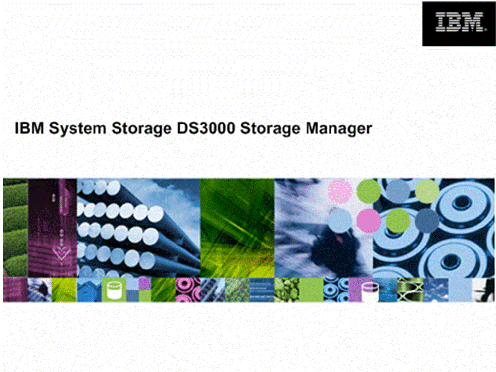
\includegraphics[width=10cm]{include/img/ds3400_1}
    \end{center}
    \caption{Ecrã inicial do StorageManager}
    \label{fig:ds3400-1}
\end{figure}

Depois deve carregar com o botão direito sobre a storage e escolher "Manage Storage Subsystem"

\begin{figure}[H]
    \begin{center}
        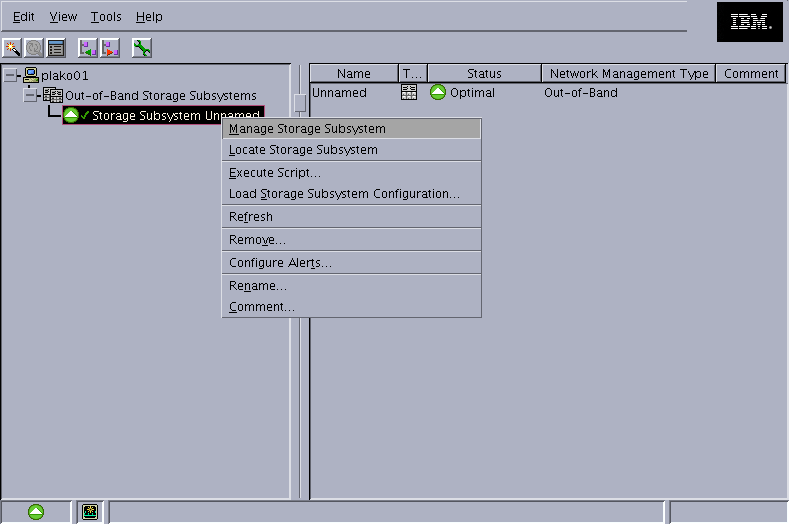
\includegraphics[width=10cm]{include/img/ds3400_2}
    \end{center}
    \caption{Ecrã principal do StorageManager}
    \label{fig:ds3400-2}
\end{figure}

Posteriormente poderá efectuar a gestão da storage. Também pode consultar o estado da storage via linha de comandos com:

\begin{Output}[commandchars=\\\{\}]
/opt/IBM\_DS/client/SMcli <IP\_DA\_STORAGE>  -c "show storageSubsystem healthStatus;"
Performing syntax check...

Syntax check complete.

Executing script...

Storage Subsystem health status = optimal.
Script execution complete.

SMcli completed successfully.
\end{Output}
